\documentclass[11pt]{jreport}
\usepackage{wuse_thesis}
\usepackage{indentfirst}
\usepackage{url}	% \url{}コマンド用.URLを表示する際に便利
\usepackage{otf}
\usepackage{xcolor}
\usepackage[dvipdfmx]{graphicx}
\usepackage{enumitem}
\usepackage{float} % 図表の強制的な配置設定が可能な[H]を使用可能にする
            
\newcommand{\RQOne}{レビューコメントの中から修正要求を抽出することは可能か}
\newcommand{\RQTwo}{レビューコメントの中から修正確認を抽出することは可能か}
\newcommand{\RQThree}{コードレビュー票単位と修正要求単位に基づくタスクの完了状況評価結果は異なるか}

\newcommand{\todo}[1]{\colorbox{yellow}{{\bf TODO}:}{\color{red} {\textbf{[#1]}}}}
\newcommand{\change}[1]{\colorbox{green}{{\bf CHANGE}:}{\color{blue} {\textbf{[#1]}}}}
\newcommand{\new}[1]{\colorbox{cyan}{{\bf NEW}:}{\color{black} {\textbf{[#1]}}}}
%%%%%%%%%%%%%%%%%%%%%%%%%%%%%%%%%%%%%%%%%%%%%%%%%%%%%%%%%%%%%%%%%%%%%%%%

%%
%% 主に表紙を作成するための情報
%%

%%  タイトル(修論の場合は英語表記も指定)
\title{修正要求・確認コメントの自動抽出による\\
コードレビューのタスク完了状況追跡手法}

%%  著者名(修論の場合は英語表記も指定)
\author{川\UTF{FA11} 晴斗}

%% 卒業論文
\bachelar	% 卒業論文(4年生用)

%%  学科・クラスタ
\department{システム工}

%%  学生番号
\studentid{60266083}

%%  卒業年度
\gyear{2024}

%%  論文提出日
\date{2025年2月12日}

%%%%%%%%%%%%%%%%%%%%%%%%%%%%%%%%%%%%%%%%%%%%%%%%%%%%%%%%%%%%%%%%%%%%%%%%

\begin{document}

\maketitle

%%
%%  概要
%%

\begin{abstract}
本研究では,コードレビューにおけるレビューコメントがソフトウェアの開発プロセスに及ぼす影響を調査する.

ソフトウェア開発において,検証者は実装者が提出したソースコードに対して,可読性や欠陥の有無の確認を行い,次回のリリースへの導入の可否を決定する.この際,レビュー対象のソースコード,検証者と実装者間のやり取り,および修正履歴を記録・管理するために,コードレビュー票が用いられる.コードレビュー票には,検証者からの指摘事項や実装者の対応状況などレビューに関する一連の情報が時系列で記録される.大規模プロジェクトでは実装者から提出されるソースコードが膨大であるため,従来研究ではソースコードが提出された際にコードレビューの優先順位や工数の見積もりを行う手法を提案している.しかし,コードレビューにおいて,検証者と実装者の間でソースコードの修正に関する意見が対立し,予定時間を超過することも多い.

本研究では,レビューコメントの内容を詳細に分析し,個々のコードレビュー票のタスクの完了状況を追跡する手法を提案する.具体的には,ソースコードの修正を要求するコメント(以降,修正要求)と修正完了を確認するコメント(以降,修正確認)を自動で抽出し,これらを対応づけることで,各修正要求の対応状況を追跡する.

提案手法の有効性を検証するため,まず自然言語処理モデルのBERTとパターンマッチを用いて修正要求と修正確認の自動抽出を試みた.その結果,修正要求についてはF値0.81,修正確認についてはF値0.96という高い精度での抽出が可能であることを確認した.次に,時系列に基づいて修正要求と修正確認の紐付けを行った結果,修正要求の86.6\%について対応する修正確認との紐付けに成功した.

本手法により,従来は困難であった個々のコードレビュー票のタスクの完了状況を詳細に追跡することが可能となり,ソフトウェアの開発プロセスの効率化に寄与することを期待する.
\end{abstract}

%%  目次
\tableofcontents

\newpage
\pagenumbering{arabic}	% 以降のページ番号を算用数字に

%%%%%%%%%%%%%%%%%%%%%%%%%%%%%%%%%%%%%%%%%%%%%%%%%%%%%%%%%%%%%%%%%%%%%%%%

%%
%%  本文はここから
%%

%%%%%%%%%%%%%%%%%%%%%%%%%%%%%%%%%%%%%%%%%%
%1章 はじめに
\chapter{はじめに}\label{chap:intro}
%%%%%%%%%%%%%%%%%%%%%%%%%%%%%%%%%%%%%%%%%%

オープンソースソフトウェア(OSS: Open Source Software)は,著作権者が定めたライセンスによってソフトウェアの変更・配布の権利が規定され,ソースコードが公開されているソフトウェアである.OSSのソースコードは,そのライセンスの条件下で,誰でも自由に利用,修正,機能の拡張,再配布を行うことが可能である\cite{oss}.

不特定多数の実装者が参加するOSS開発では複数の開発者(実装者)がソフトウェアの機能の追加や不具合修正のために,変更したソースコードをプロジェクトに提出する.変更したソースコードは別の開発者(検証者)によってコードレビューが実施される.コードレビューは変更したソースコードに欠陥の有無やコードの可読性を損失する箇所が存在しないかを確認する重要な工程である\cite{quality1}\cite{quality2}.コードレビューによってソースコードの改善を要する箇所が発見されれば,検証者は実装者に改善を要求する. 

さらに,コードレビューはプロジェクトのリリースに直接影響を与える重要な要素の一つである.コードレビューの議論を通じて,変更されたソースコードがプロジェクトへの導入に適した水準を満たしていると判断された場合,次回のリリースへの導入が決定される.ソフトウェア開発プロジェクトでは,リリースまでのマイルストーンを計画するために,コードレビューを含めた各タスクの進捗を計画し,完了状況を追跡する必要がある\cite{review_time}.この進捗確認のため,ソースコードの共有や管理を行うサービスであるGitHub\footnote{GitHub: \url{https://github.co.jp/}}はMilestone機能を提供している.この機能により,特定の期限までに完了すべきコードレビュー(Pull Request)票の件数を把握することが可能となるため,多くの組織がリリースまでのマイルストーン管理に活用している.ただし,コードレビューの過程では,実装者と検証者の間でソースコードの修正の必要性について対立し,レビューの完了の予定時間を超過することが多い\cite{review_time1}\cite{review_time2}.そのため,緻密なマイルストーンを計画するためには,個々のコードレビュー票に含まれるレビューのタスクの完了状況を正確に追跡する必要がある.しかしながら,OSS開発では提出されるコードレビュー票が膨大であるため,個々のコードレビュータスクの完了状況を追跡することは困難である.

本研究では,コードレビューにおけるタスクの完了状況の把握に向けて,実装者と検証者の議論の中から,検証者がコードレビューによって更なる修正を依頼するコメント(以降,修正要求),およびソースコードが修正されたことを検証者が確認したことを伝えるコメント(以降,修正確認)を自動抽出する手法を提案する.また,GitHubのMilestoneのようなコードレビュー票単位でのタスクの完了状況追跡手法と,本研究で開発する修正要求単位でのタスクの完了状況追跡手法の違いを示す.

\noindent\textbf{RQ1: \RQOne (\ref{chap:RQ1}章)}\\
RQ1では,検証者が記録するコードレビュー票に残したレビューコメントを修正要求に分類できるか否かを調査する.具体的には,OSS開発で公開されているコードレビュー票を無作為に抽出し,各コードレビュー票に記録されたレビューコメントについて目視,及び機械的に分類を行う.

\noindent\textbf{RQ2: \RQTwo (\ref{chap:RQ2}章)}\\
RQ2では,検証者が記録するコードレビュー票に残したレビューコメントを修正確認に分類できるか否かを調査する.具体的には,RQ1で無作為に抽出したコードレビュー票において,各コードレビュー票に記録されたレビューコメントについて目視,及び機械的に分類を行う.

\noindent\textbf{RQ3: \RQThree (\ref{chap:RQ3}章)}\\
RQ3では,修正要求とその要求が解決されたことを確認する修正確認の紐付けを試みる.また,従来のコードレビュー票に基づいた手法と本研究で開発した修正要求に基づいた手法によるコードレビューのタスクの完了状況の追跡結果の違いを示す.

以降,本論文では,\ref{chap:review_process}章でOSS開発におけるコードレビューと従来研究について述べる.その後,\ref{chap:case_study}章で本研究の概要やデータセットについて述べ,\ref{chap:RQ1}章でRQ1,\ref{chap:RQ2}章でRQ2,\ref{chap:RQ3}章でRQ3のそれぞれの手法と結果について述べる.そして\ref{chap:discussion}章で結果の考察及び妥当性について述べ,\ref{chap:conclusion}章でまとめる.

%%%%%%%%%%%%%%%%%%%%%%%%%%%%%%%%%%%%%%%%%%
%2章 コードレビュープロセス
\chapter{コードレビュープロセス}\label{chap:review_process}
%%%%%%%%%%%%%%%%%%%%%%%%%%%%%%%%%%%%%%%%%%

\section{コードレビュー}
ソフトウェア開発において,開発者(実装者)は自身が実装した機能追加や不具合を修正するためのソースコードをプロジェクトに向けて提出する.別の開発者(検証者)は,コードレビューという開発プロセスによって,提出されたソースコードを評価する.コードレビュープロセスでは3つのプロセスを経てプロジェクトへ導入,および却下の判断が検証者によって下される.

\begin{enumerate}[label=\textbf{ステップ\arabic*:}, leftmargin=75pt]
\item 検証者は提出されたソースコードに対してコードレビューを行う.また,以前のコードレビューにおいて,修正要求が行われている場合については,変更箇所を確認し,問題がなければ修正確認のコメントを投稿する.
\item コードレビューにより,プロジェクトへの有用性の有無やプロジェクトに導入可能な水準を満たしているかなどの観点から導入,却下,およびソースコードに対して修正要求を投稿のいずれかを決定する.
\item 修正要求が投稿された場合,実装者は修正要求に基づいて変更を行い,再度ソースコードを提出する.
\end{enumerate}

また,図\ref{fig:code_review}はレビュー管理システムGerritのコードレビュー画面\footnote{\url{https://review.opendev.org/c/openstack/nova/+/1543}}を示す.コードレビューでは修正要求および修正確認の投稿が複数回にわたって行われ,プロジェクトのソースコードの品質を維持,向上させている.

%-------------------
\begin{figure*}[t]
\centerline{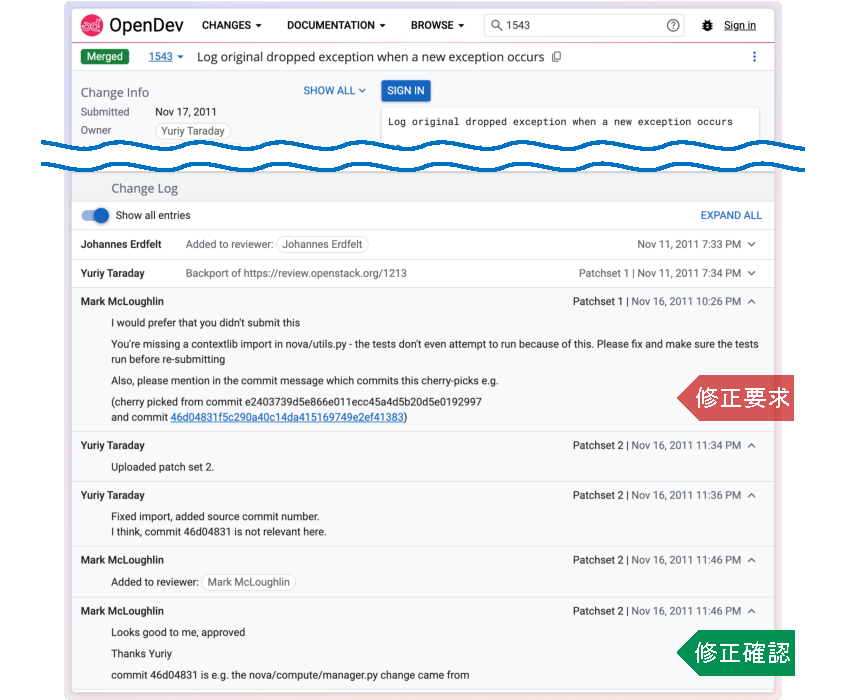
\includegraphics[width=1.0\linewidth]{@BSthesis2024_Kawasaki/BSthesis2024_Kawasaki_fig/code_review.pdf}}
\caption{Gerritのコードレビュー画面}
\label{fig:code_review}
\end{figure*}
%-------------------

検証者が導入の判断を下したソースコードについては,次回のリリースに含められるため,コードレビューはソフトウェア開発のリリースに重要な影響を与える.ソフトウェア開発プロジェクトでは,リリーススケジュールに合わせて図\ref{fig:milestone}のように\footnote{\url{https://github.com/microsoft/vscode/milestone/288}}コードレビューを含めたマイルストーンが計画される.ただし,提出されたソースコードの修正の必要性について,他の検証者,または実装者同士で意見が対立し,コードレビューの時間が長期化することも多い\cite{review_time1}\cite{review_time2}.

そのため,より正確なマイルストーンを計画するためにコードレビューに含まれる議論の内容を追跡することが望まれるが,OSS開発では日々膨大な量のソースコードが提出されるため,個々の議論の内容を追跡することは難しい.また,議論に含まれるレビューコメントが修正要求であるか否か,および修正要求が満たされているかを検証者が確認しているか否かの判断を行うための指標が存在しないため,コードレビューのタスクの完了状況を自動で追跡することは容易ではない.

%-------------------
\begin{figure*}[t]
\centerline{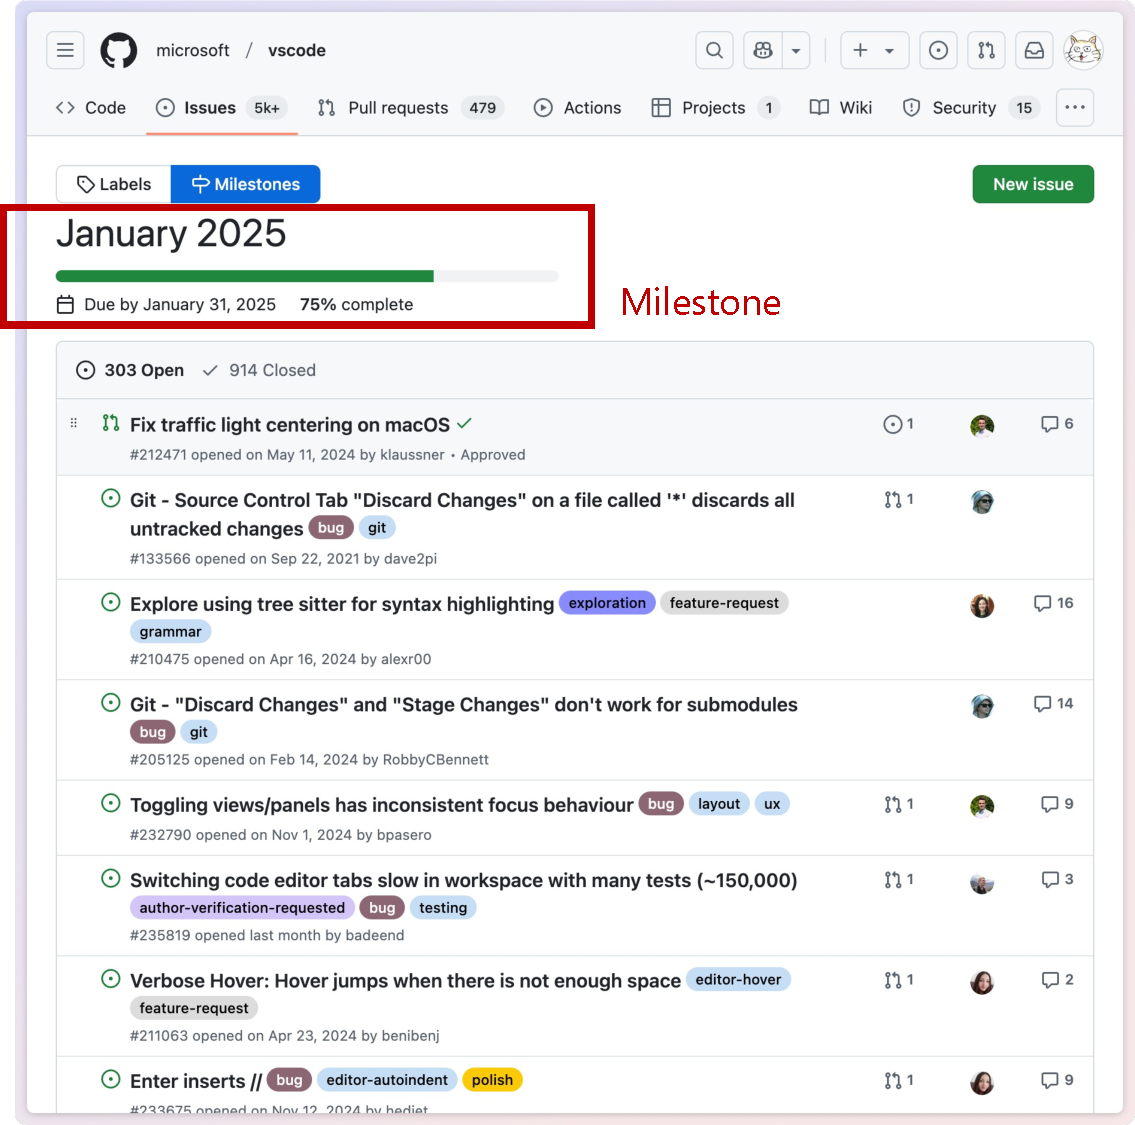
\includegraphics[width=0.9\linewidth]{@BSthesis2024_Kawasaki/BSthesis2024_Kawasaki_fig/milestone.pdf}}
\caption{GitHubのMilestoneの画面}
\label{fig:milestone}
\end{figure*}
%-------------------

\section{関連研究}
大規模OSSの開発では,実装者がコードレビュー依頼をGerritやReview Boardをはじめとしたコードレビュー管理システムの票に記録することで,実装者と検証者が円滑なコミュニケーションを行う~\cite{code_review}.これらのシステムに蓄積されたデータを用いて,コードレビューの作業内容や工数を見積もる研究が行われている.

大規模OSSの開発では,日々膨大なコードレビュー票がプロジェクトに提出されるため,開発者は優先して取り組むコードレビュー票に順位をつけて作業を効率化している.従来研究ではコードレビュー票の優先順位を決定するための研究が多数存在しており,ソフトウェア利用者に悪影響を与えるセキュリティ関連の不具合を修正するソースコードのコードレビューは優先順位が高く設定されることが明らかにされている~\cite{integrator}\cite{review_prioritize_pineapple}.また,その他の急を要さない不具合修正やリファクタリングのために変更されたソースコードのコードレビューは優先順位が日々変動する\cite{review_priority_next_day}.

コードレビューの進捗を計画,追跡することは,リリースまでの緻密なマイルストーンを計画するために重要であり,各コードレビューに要する時間を見積もる研究が行われている.
Maddilaらは,レビューに参加している検証者の数やソースコードが提出された曜日など,レビューの完了時間に影響を与える要素を調査し,完了時間を予測するモデルを作成した\cite{estimate_time1}\cite{estimate_time2}.Chouchenらは,コードレビューに関する69個の要素から回帰分析を行い,レビューの完了時間を予測するモデルを作成した\cite{estimate_time3}.Jonathanらは検証者のレビューステータスを調査することでレビューにかかる時間を調査し,レビュー依頼を投稿したソースコード提案は依頼を投稿していないソースコード提案よりレビュー時間が短くなることを明らかにした\cite{estimate_time4}.Manoelらは,複数の回帰手法から最もレビュー時間の予測に適した手法を明らかにした\cite{estimate_time5}.Kononenkoらは,開発者へのインタビューにおいて,コード行数やコメントした検証者の数はコードレビューにかかる時間に影響を及ぼすことを明らかにした\cite{release_merge}.

従来研究ではコードレビューの優先順位,およびコードレビューにかかる工数の見積もりにコードレビュー票を提出した時点で計測可能な特徴量に基づいていることが多い.本研究ではレビューコメント内で検証者によって投稿されている修正要求,および修正要求の完了度合いを抽出することで動的なタスクの完了状況の追跡を可能にする.

\section{動機}
ソフトウェア開発ではリリーススケジュールに合わせてマイルストーンを計画する.OSS開発では実装者から膨大な量のソースコードが提出されるため,従来研究ではコードレビュー票が提出された時点で,優先順位や工数の見積もりを行う手法を提案している~\cite{estimate_time1}\cite{estimate_time2}\cite{estimate_time3}\cite{estimate_time4}\cite{estimate_time5}.しかし,コードレビューでは他の検証者や開発者同士で意見が対立することもあり,マイルストーンで予定していたコードレビューの時間を超過することも多い\cite{review_time1}\cite{review_time2}.そのため,より緻密なマイルストーンを計画するためには,個々のコードレビュー票のタスクの完了状況を追跡する必要がある.

本研究では,個々のコードレビュー票のタスクの完了状況を追跡するために,レビューコメントに含まれる修正要求の完了状況を自動で抽出することは可能であるかを検証する.具体的には,コードレビュー票に投稿されたレビューコメントから修正要求と修正確認を自動で抽出し,それぞれを対応したコメント同士で紐づけることは可能であるかを検証する.

\section{リサーチクエスチョン}
本論文では,3つのRQを設定し,検証することで本研究の追跡手法がコードレビューのタスクの完了状況の追跡に有効であるかを評価する.

\vskip\baselineskip
\noindent\textbf{RQ1:\RQOne}

レビューコメントには提出されたソースコードに対する修正要求のコメント以外にも,他の開発者への質問や,修正要求が解決したことの確認など多種多様なコメントが投稿されている.RQ1では,これらのレビューコメントから修正要求を高い精度で自動抽出することが可能であるかを調査する.

\vskip\baselineskip
\noindent\textbf{RQ2:\RQTwo}

RQ1と同様にレビューコメントには多種多様なコメントが投稿されているため,RQ2ではレビューコメントから修正確認を高い精度で自動抽出可能であるかを調査する.

\vskip\baselineskip
\noindent\textbf{RQ3:\RQThree}

コードレビューにおいて,開発者同士で意見が対立する場合は長期化することもあるため,従来手法のコードレビュー票を用いた手法では正確なタスクの完了状況を追跡することは難しい.本研究では,レビューコメントに含まれる修正要求を用いたタスクの完了状況追跡手法によって,従来のコードレビュー票に基づくタスクの完了状況追跡手法と評価結果が異なるかを調査する.

%%%%%%%%%%%%%%%%%%%%%%%%%%%%%%%%%%%%%%%%%%
%3章ケーススタディ
\chapter{ケーススタディ}\label{chap:case_study}
%%%%%%%%%%%%%%%%%%%%%%%%%%%%%%%%%%%%%%%%%%

\section{概要}
コードレビューでは複数の開発者からソースコードへの修正要求や,提出されたソースコードへの問い,修正要求が解決したことの確認など多岐にわたるコメントが投稿されている.コードレビューにおけるタスクの完了状況の把握を行うためには,ソースコードに対する修正要求がどの程度完了しているかを抽出する必要がある.したがって,本研究ではレビューコメントの投稿数が多い,OpenStackのプロジェクトを対象としてレビューコメントに含まれる修正要求の完了度合いを抽出することでコードレビューのタスクの完了状況の追跡を行う.

本研究で用いる手法を図\ref{fig:research_method}に示す.RQ1では,図\ref{fig:research_method}の中央上部に示すようにレビューコメントから修正要求を自動で抽出することが可能かを検証する.まず,レビューコメントにおいて,目視で修正要求か否かを分類する.次に,目視で分類したデータセットから作成した自然言語処理モデルのBERTを用いて,レビューコメントから修正要求を自動で抽出することが可能かを検証する.

RQ2では図\ref{fig:research_method}の右上部に示すようにレビューコメントから修正確認を自動で抽出することが可能かを検証する.まず,レビューコメントにおいて,目視で修正確認か否かを分類する.次に目視で分類したデータセットから得られた知見をもとにパターンマッチを行い,レビューコメントから修正確認を自動で抽出することが可能かを検証する.

RQ3では図\ref{fig:research_method}の下部に示すように修正要求と修正確認を対応したコメント同士で紐付け,修正要求の完了と未完了を分類することが可能かを検証する.まず,RQ1,およびRQ2での手法を用いてレビューコメントから修正要求と修正確認を自動で抽出する.次に,修正要求と修正確認を紐づけるための定義を作成し,修正要求と修正確認を自動で紐付け可能かを検証する.

%-------------------
\begin{figure*}[t]
\centerline{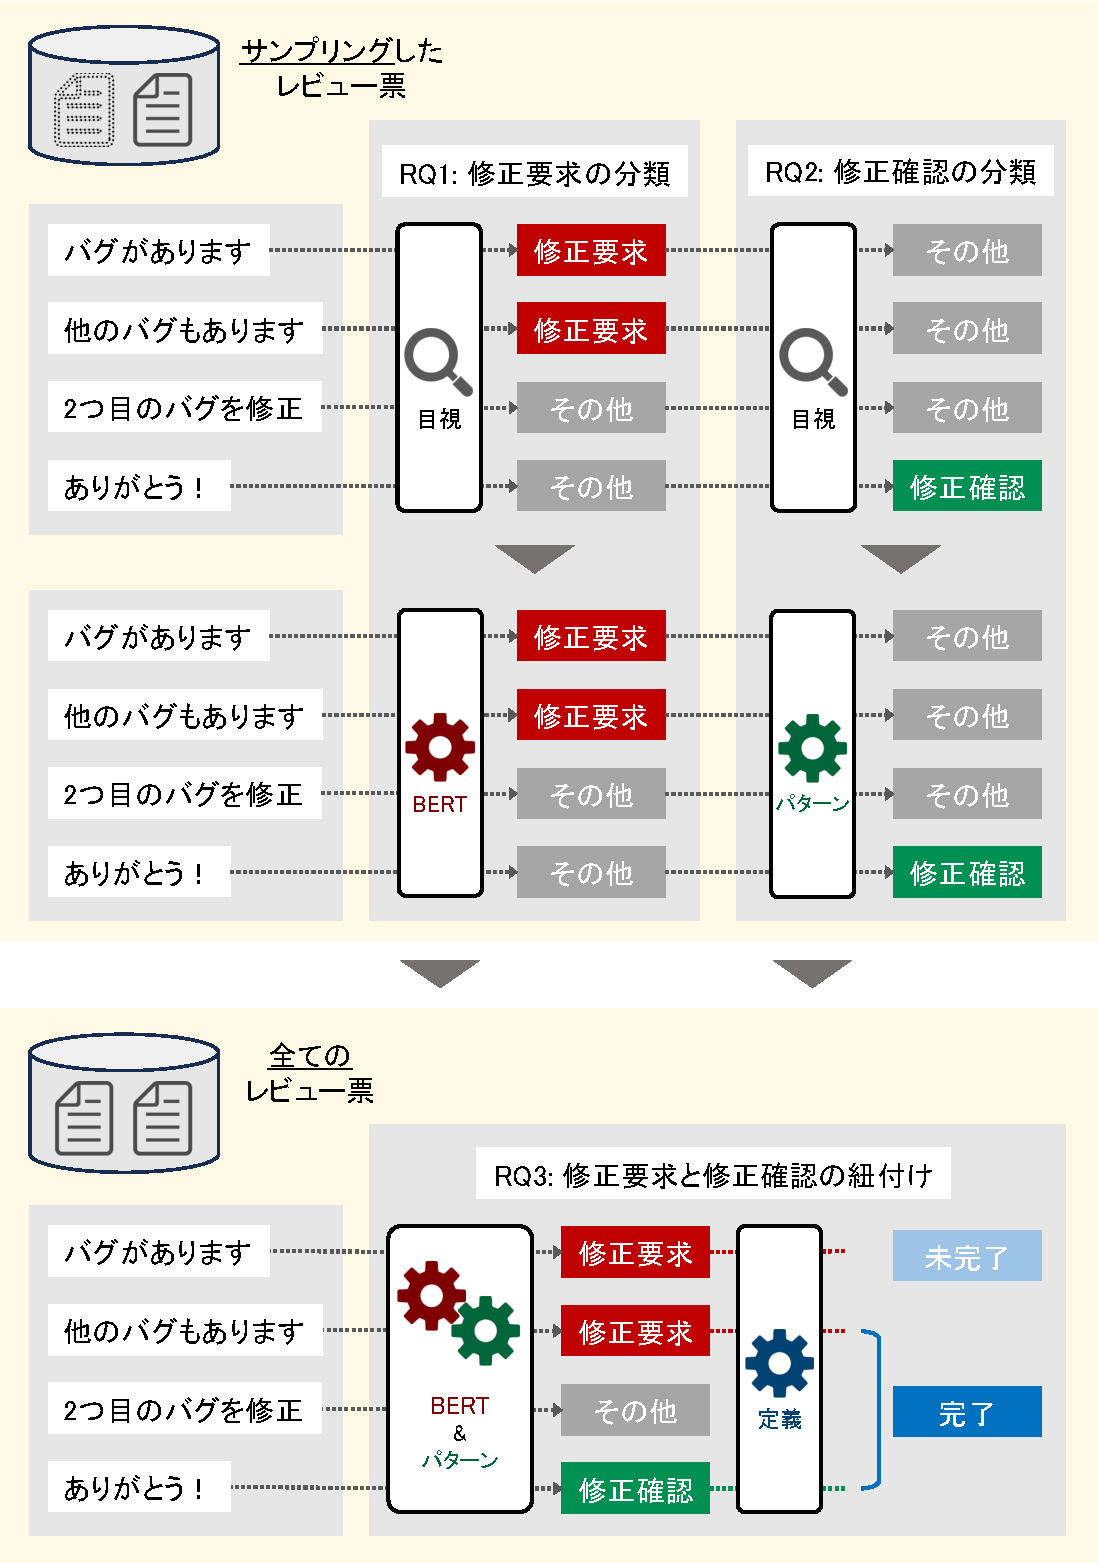
\includegraphics[width=1.00\linewidth]{@BSthesis2024_Kawasaki/BSthesis2024_Kawasaki_fig/research_method.pdf}}
\caption{コードレビューのタスクの完了状況追跡手法}
\label{fig:research_method}
\end{figure*}
%-------------------

また,BERT,およびパターンマッチを用いた手法での修正要求,または修正確認の抽出精度の評価指標として適合率,再現率,F値を用いる.評価指標の算出にあたって,両手法での抽出結果を4つに分類する.

\begin{itemize}
\item \textbf{True Positive(TP)}: 目視調査にて修正要求/修正確認と分類したレビューコメントに対して,修正要求/修正確認と正しく予測するケース
\item \textbf{False Positive(FP)}: 目視調査にて非修正要求/非修正確認と分類したレビューコメントに対して,修正要求/修正確認と誤って予測するケース
\item \textbf{True Negative(TN)}: 目視調査にて非修正要求/非修正確認と分類したレビューコメントに対して,非修正要求/非修正確認と正しく予測するケース
\item \textbf{False Negative(FN)}: 目視調査にて修正要求/修正確認と分類したレビューコメントに対して,非修正要求/非修正確認と誤って予測するケース
\end{itemize}

適合率は,式\ref{formula:precision}に示すように,修正要求/修正確認と予測したレビューコメントの中で,目視調査にて修正要求/修正確認と分類したレビューコメントの割合を表す.適合率は0から1の間で算出され,値が大きいほど予測の精度が高いことを表す.

%-----------------------
\begin{equation}
適合率 = \frac{TP}{TP+FP}\label{formula:precision}
\end{equation}
%-----------------------

再現率は,式\ref{formula:recall}に示すように,目視調査にて修正要求/修正確認と分類したレビューコメントの中で,修正要求/修正確認と予測したレビューコメントの割合を表す.再現率は0から1の間で算出され,値が大きいほど予測の精度が高いことを表す.

%-----------------------
\begin{equation}
再現率 = \frac{TP}{TP+FN}\label{formula:recall}
\end{equation}
%-----------------------

F値は,式\ref{formula:f_score}に示すように,適合率と再現率の調和平均を表す.F値は0から1の間で算出され,値が大きいほど予測の精度が高いことを表す.

%-----------------------
\begin{equation}
F値 = 2*\frac{適合率*再現率}{適合率+再現率}\label{formula:f_score}
\end{equation}
%-----------------------

\section{データセット}
OpenStackプロジェクトでは,レビュー管理システムとしてGerritを使用しており,各コードレビュー票における開発者からのコメント投稿数が多いため,多くの従来研究がコードレビュー過程を分析するための調査対象としている.そこで本研究では,OpenStackのコアコンポーネントであるNova,Neutron,Cinder,Keystone,Swift,Glanceの6つのプロジェクト,およびOpenStackにおける大規模プロジェクトであるHorizonの合計7つのプロジェクトのうち,プロジェクトの立ち上げから2023年5月までにリポジトリに導入されたコードレビュー票に記録されるレビューコメントを分析対象とする.表\ref{table:sum_of_projects}は,各プロジェクトのコードレビュー票数,コメント数を示す.プロジェクト毎のコードレビュー票の平均コメント数は22件から87件であり,それぞれのコードレビュー票には多数のレビューコメントが投稿されていることが確認できる.

%-----------------------
\begin{table}[t]
\centering
  \caption{各プロジェクトにおいて導入されたコードレビュー票数とコメント数}
  \vspace{+1mm}
  \label{table:sum_of_projects}
  \scalebox{0.9}{   
  \begin{tabular}{l|r|r}  \hline \hline
    \multicolumn{1}{c|}{プロジェクト} & \multicolumn{1}{c|}{コードレビュー票数} & \multicolumn{1}{c}{コメント数}\\ \hline
    Nova & 29,338 & 1,571,114\\ 
    Neutron & 18,665 & 1,106,829\\ 
    Cinder & 12,917 & 1,127,176\\ 
    Horizon & 9,645 & 209,681\\ 
    Keystone & 8,270 & 190,464\\ 
    Swift & 6,172 & 112,709\\ 
    Glance & 4,545 & 102,360\\ \hline
    合計 & 89,552 & 4,420,333\\ \hline
  \end{tabular}
  }
\end{table}
%-----------------------

%%%%%%%%%%%%%%%%%%%%%%%%%%%%%%%%%%%%%%%%%%
%4章 RQ1
\chapter{RQ1:\RQOne}\label{chap:RQ1}
%%%%%%%%%%%%%%%%%%%%%%%%%%%%%%%%%%%%%%%%%%

\section{概要}
RQ1では,本研究で用いるデータセットのうち無作為に選択した一部のコードレビュー票に記録されたレビューコメントの中から,修正要求を抽出することが可能か否かを目視調査する.また,目視調査で作成した修正要求か否かを分類したデータセットを用いて,自然言語処理モデルのBERTをファインチューニングし,レビューコメントから修正要求を抽出するモデルの構築と評価を行う.

\section{手法}
\subsection{目視での分類手法}\label{subsec:request_manual_method}
分析対象とする7プロジェクトを区別せずに89,552件のコードレビュー票から信頼区間95\%,許容誤差5\%となる383件を無作為に選択し,選択したコードレビュー票に投稿されたレビューコメント12,086件を本研究の著者が目視調査する.具体的には投稿されたコメントが修正要求のコメントか否かを分類する.なお,コードレビューにおいては,ソースコードのビルド結果の確認など,自動化されたボットによるコメントが含まれることがある.実装者がこれらボットのコメントに全て対処する前に検証者がソースコードを導入することもあるため,本研究ではボットによるコメントは修正要求の対象から除外する.

\subsection{BERTでの分類手法}
自然言語処理モデルのBERT\footnote{BERT: \url{https://huggingface.co/docs/transformers/ja/model_doc/bert}}において,\ref{subsec:request_manual_method}項で目視調査したデータセットを教師データとして用いてファインチューニングを行い,レビューコメントに含まれる修正要求の抽出と評価を行う.具体的には目視調査した12,086件のレビューコメントを5分割し,1つをテスト用のデータに用いて,残りの4つを訓練用のデータに用いる5分割交差検証を行う.訓練用のデータは,さらに7:3の割合で分割して学習用と検証用のデータとして用いる.モデル作成時のパラメータは学習時のパッチサイズが8,評価時のパッチサイズが16,エポック数が3,ウォームアップステップ数が500,重み減衰が0.01とした.評価指標には適合率,再現率,F値を用い,交差検証で5回実行した結果の中央値でモデルの有用性を評価する.

また,Gerritでは検証者がコードレビューのコメントに検証の評価結果を表すラベルの付与を示す機能を有しており,変更内容に賛成していることを表すラベルとして\textit{``Looks good to me, approved(Code-Review+2)''}や\textit{``Looks good to me, but someone else must approve(Code-Review\\+1)''},変更内容に反対していることを表すラベルとして\textit{``I would prefer that you didn't submit this(Code-Review-1)''}や\textit{``I would prefer that you didn't merge this(Code-Review-2)''}などがある.これらの検証評価ラベルが修正要求の抽出に与える影響を確認するため,同様の設定のモデルを用いて,検証評価ラベルが付与されたレビューコメントからラベルを削除したコメントだけをテストデータに用いて評価も行う.

さらに,BERTが自然言語による要求表現を適切に理解できているかを確認するために,目視調査した12,086件のレビューコメントから前処理を行った6,049件のレビューコメントに含まれる頻出単語を調査する.前処理では,ボットによるコメントを分析対象から除外し,残りのコメントから検証評価ラベル,プロジェクト名(Nova,Neutron,Cinder,Horizon,Keystone,Swift,Glance),URL,数字,記号を削除した.

\section{結果}
\subsection{目視での分類結果}\label{subsec:request_manual_result}
表\ref{table:request_sum}は,分析対象とする12,086件のレビューコメントから修正要求か否かを内容に基づき目視分類した結果を示す.レビューコメントのうち,874件(約7.2\%)が修正要求であり,それぞれの修正要求は5パターン(機能改善,リファクタリング,コード外の修正,バグ修正,誤字修正)に分類可能なことを確認した.機能改善やコード外の修正,バグ修正は表~\ref{table:request_sum}に示す以外にも\textit{``Needs unit tests.''}や\textit{``This could use a bit more explanation in the commit message.''},\textit{``Fix the bug.''}のように\textit{``need''},\textit{``could''},\textit{``fix''}などの自然言語で一般的に要求や修正を表す単語が多く用いられていることを確認した.また,リファクタリングや誤字修正には他の修正要求に比べてコメントに含まれる単語の量は少ないが,表~\ref{table:request_sum}に示す\textit{``instead''}のような単語や\textit{``-\textgreater''}のように定型的な表現を用いて変更を示していることが多いことを確認した.

これらの結果からレビューコメントにおける修正要求には特徴があることを確認したため,修正要求は機械的な手法でレビューコメントから抽出できる可能性が高いことが示唆される.

%-----------------------
\begin{table*}[t]
\centering
  \caption{修正要求に含まれていた内容}
  \label{table:request_sum}
  \scalebox{0.78}{   
  \begin{tabular}{l|l|r}  \hline \hline
    \multicolumn{1}{c|}{修正要求内容} & \multicolumn{1}{c|}{コメント例} & \multicolumn{1}{c}{件数(重複可)}\\  \hline
    機能改善 & better to use mock instead of stub & 345\\
    リファクタリング/コード整形 & Could you use rstrip instead? & 278\\ 
    コード外の修正(コミットメッセージ等) & commit message line should have less than 72 characters & 233\\ 
    バグ修正 & need to address failures in unit tests & 92\\ 
    誤字修正 & fileds -\textgreater fields & 47\\  \hline
  \end{tabular}
  }
\end{table*}
%-----------------------

\subsection{BERTでの分類結果}
表\ref{table:request_score}は,BERTにファインチューニングしたモデルを用いてレビューコメントから修正要求を抽出した結果を示す.5分割交差検証の結果,適合率0.84,再現率0.78,F値0.81となった.この結果からレビューコメントから修正要求を高い精度で抽出することが可能であることを明らかにした.

%-----------------------
\begin{table}[t]
\centering
  \caption{修正要求の予測精度}
  \label{table:request_score}
  \scalebox{1.00}{   
  \begin{tabular}{l|r|r|r}  \hline \hline
    \multicolumn{1}{c|}{スコア(件数)} & \multicolumn{1}{c|}{適合率} & \multicolumn{1}{c|}{再現率} & \multicolumn{1}{c}{F値}\\ \hline
    全レビューコメント(12,086件) & 0.84 & 0.78 & 0.81\\ \hline    
  \end{tabular}
  }
\end{table}
%-----------------------

また,表\ref{table:metrics_recall}は,\ref{subsec:request_manual_result}項にて分類した修正要求内容別の再現率を示す.修正要求内容が200件以上存在する機能改善,リファクタリング/コード整形は,再現率が8割以上であることを確認した.一方で,コード外の修正やバグ修正,誤字修正は機能改善やリファクタリング/コード整形と比べると再現率が低下した.この理由としては,コード外の修正はコミットメッセージの修正や変更に対するパッチの分割要求など,修正要求の対象が多岐に渡っていることが起因していると示唆する.また,バグ修正や誤字修正は,データセットの中に含まれる修正要求が少ないことが再現率の低下に起因していると示唆する.ただし,全ての修正要求内容の再現率が7割以上であることから修正要求内容の種類によらず,レビューコメントから修正要求を高い精度で抽出できていることが確認できる.

%-----------------------
\begin{table}[t]
\centering
  \caption{修正要求内容毎の再現率}
  \label{table:metrics_recall}
  \scalebox{1.0}{
  \begin{tabular}{l|r}  \hline \hline
    \multicolumn{1}{c|}{修正要求内容} & \multicolumn{1}{c}{再現率}\\ \hline
    機能改善(345件) & 0.81\\ 
    リファクタリング/コード整形(278件) & 0.85\\ 
    コード外の修正(233件) & 0.76\\ 
    バグ修正(92件) & 0.74\\ 
    誤字修正(47件) & 0.79\\ \hline
  \end{tabular}
  }
\end{table}
%-----------------------

次に,表\ref{table:label_less_score}は,検証評価ラベルが付与されたレビューコメントからラベルを削除したコメントだけをテストデータに用いた評価結果を示している.Code-Review-2は適合率,F値ともに低いが,これはラベルを含むコメントが14件と少量であることから評価指標の値にばらつきが生じたことが示唆される.Code-Review-1は修正要求を含むコメントが多量に存在しているため,全ての評価指標が高いことがわかる.Code-Review+1,およびCode-Review+2は修正要求において承認を示すラベルであるが,時にコメントに修正要求を併記していることもある.そのため,他の検証評価ラベルやラベルが付与されていないコメントに比べて,コメントから修正要求を抽出することは困難であることがわかるが,全ての評価指標でどちらも6割を超えている.これらの結果から,コメントの件数が少なかったCode-Review-2を除いて,検証評価ラベルが付与されたコメントからラベルを削除したとしても,F値が6割以上あることは,BERTがラベルなしでも自然言語による要求表現を適切に理解できていることが示唆される.

%-----------------------
\begin{table}[t]
\centering
  \caption{検証評価ラベルを除いたコメントに含まれる修正要求の予測精度}
  \label{table:label_less_score}
  \scalebox{1.00}{   
  \begin{tabular}{l|r|r|r}  \hline \hline
    \multicolumn{1}{c|}{検証評価ラベル(件数)} & \multicolumn{1}{c|}{適合率} & \multicolumn{1}{c|}{再現率} & \multicolumn{1}{c}{F値}\\ \hline 
    Code-Review-2(14件) & 0.20 & 1.00 & 0.33\\ 
    Code-Review-1(465件) & 0.97 & 0.97 & 0.96\\ 
    Code-Review+1(918件) & 0.78 & 0.70 & 0.69\\ 
    Code-Review+2(916件) & 0.60 & 0.64 & 0.63\\ \hline
  \end{tabular}
  }
\end{table}
%-----------------------

表\ref{table:word_frequency}は著者,およびBERTが分類したレビューコメントに頻出する単語の上位10件を示している.著者が分類した結果では修正要求の上位に,要求を表す\textit{``need''}や要求表現の一部である\textit{``would''},\textit{``like''},変更を意味する\textit{``change''}などが含まれていることを確認できる.同様に著者が分類した結果では非修正要求の上位に,ボットに対してビルドのテストを命令する\textit{``recheck''}やソースコードの修正の確認を表す際に用いる\textit{``thanks''},確認表現の一部である\textit{``look''},\textit{``good''}などが含まれていることを確認できる.これらの著者が分類したレビューコメントに頻出する修正要求,および非修正要求の単語はBERTの頻出単語の上位にも含まれていることから,BERTが自然言語による要求表現を適切に理解できていることを明らかにした.

%-----------------------
\begin{table}[t]
\centering
  \caption{各分類手法においてレビューコメントに頻出する単語の上位10件}
  \label{table:word_frequency}
  \scalebox{0.87}{   
  \begin{tabular}{l|r|l|r|l|r|l|r}  \hline \hline
  \multicolumn{4}{c|}{修正要求} & \multicolumn{4}{c}{非修正要求}\\ \hline
  \multicolumn{2}{c|}{著者が分類(809件)} & \multicolumn{2}{c|}{BERTが分類(758件)} & \multicolumn{2}{c|}{著者が分類(5,240件)} & \multicolumn{2}{c}{BERTが分類(5,291件)}\\ \hline
    \multicolumn{1}{c|}{単語} & \multicolumn{1}{c|}{件数(割合)} & \multicolumn{1}{c|}{単語} & \multicolumn{1}{c|}{件数(割合)} & \multicolumn{1}{c|}{単語} & \multicolumn{1}{c|}{件数(割合)} & \multicolumn{1}{c|}{単語} & \multicolumn{1}{c}{件数(割合)}\\ \hline
    need & 160(19.8\%) & need & 157(20.7\%) & recheck & 662(12.6\%) & recheck & 664(12.5\%)\\
    like & 129(15.9\%) & think & 120(15.8\%) & thanks & 260( 5.0\%) & thanks & 226( 5.0\%)\\
    test & 129(15.9\%) & like & 115(15.2\%) & patch & 228( 4.4\%) & patch & 239( 4.5\%)\\
    think & 127(15.7\%) & change & 115(15.2\%) & look & 201( 3.8\%) & look & 213( 4.0\%)\\
    change & 118(14.6\%) & comment & 113(14.9\%) & bug & 192( 3.7\%) & bug & 207( 3.9\%)\\
    would & 116(14.3\%) & test & 111(14.6\%) & test & 180( 3.4\%) & test & 198( 3.7\%)\\
    comment & 113(14.0\%) & would & 104(13.7\%) & comment & 179( 3.4\%) & comment & 179( 3.4\%)\\
    look & 109(13.5\%) & use & 103(13.6\%) & change & 171( 3.3\%) & change & 174( 3.3\%)\\
    use & 98(12.1\%) & look & 97(12.8\%) & good & 160( 3.1\%) & good & 169( 3.2\%)\\
    also & 97(12.0\%) & line & 93(12.3\%) & done & 159( 3.0\%) & done & 162( 3.1\%)\\ \hline
  \end{tabular}
  }
\end{table}
%-----------------------

%%%%%%%%%%%%%%%%%%%%%%%%%%%%%%%%%%%%%%%%%%
%5章 RQ2
\chapter{RQ2:\RQTwo}\label{chap:RQ2}
%%%%%%%%%%%%%%%%%%%%%%%%%%%%%%%%%%%%%%%%%%

\section{概要}
コードレビューにおいて,修正要求が行われた箇所の修正が完了していた際,検証者は修正確認を投稿する.本章では,修正要求や質問など多種多様なコメントが投稿されているレビューコメントから修正確認を自動で抽出することは可能かを調査する.具体的にはレビューコメントを目視で修正確認か否かに分類し,得られた知見をもとに修正確認を抽出するためのパターンマッチを行う.

\section{手法}
\subsection{目視での分類手法}
RQ1と同様に本研究で用いるデータセットのうち信頼区間95\%,許容誤差5\%の383件のコードレビュー票に投稿された12,086件のレビューコメントにおいて目視で修正確認のコメントか否かを本研究の著者が分類する.なお,RQ1と同様にボットのコメントは修正確認の対象から除外する.

\subsection{パターンマッチでの分類手法}
2つの定義のいずれかに該当する検証評価ラベルまたは語彙を含むレビューコメントを修正確認として抽出するパターンマッチを行う.評価指標には適合率,再現率,F値を用いる.

\begin{itemize}
\item Gerritで提供されている承認を示す検証評価ラベル(Code-Review+1やCode-Review+2など)
\item 修正確認と分類されたコメントの中に含まれる語彙のうち,2つの定義を同時に満たす語彙
\begin{itemize}
    \item その語彙を含むコメントが修正確認として10回以上分類されている
    \item その語彙が含まれるコメントは90\%以上の割合で修正確認として分類されている
\end{itemize}
\end{itemize}

\section{結果}
\subsection{目視での分類結果}
表\ref{table:achieve_sum} は,分析対象とする12,086件のコメントから修正確認か否か,を内容に基づき目視分類した結果を示す.12,086件のレビューコメントのうち,1,874件(約15.5\%)が修正確認であった.これらの修正確認のうち,1,559件(約83.2\%)は承認を示す検証評価ラベルがレビューコメントに付与されていることを確認した.また,検証評価ラベル以外の修正確認として,\textit{``Good Change``}や\textit{``Thank you``}などの感謝を示すコメントを投稿する検証者も複数確認した.

この結果からレビューコメントにおける修正確認には特徴があることを確認したため,修正確認は機械的な手法でレビューコメントから抽出できることが示唆される.

%-----------------------
\begin{table*}[t]
\centering
  \caption{修正確認に含まれていた内容}
  \label{table:achieve_sum}
  \scalebox{0.85}{   
  \begin{tabular}{l|l|r}  \hline \hline
    \multicolumn{1}{c|}{修正確認内容} & \multicolumn{1}{|c}{コメント} & \multicolumn{1}{|c}{件数(重複無)} \\ \hline
    強い承認 & Looks good to me, approved または Code-Review+2 & 666 \\ 
    弱い承認 & Looks good to me, but someone else must approve または Code-Review+1 & 893 \\ 
    その他 & Good Change や Thank you や Nice など & 315 \\ \hline
  \end{tabular}
  }
\end{table*}
%-----------------------

\subsection{パターンマッチでの分類結果}
表\ref{table:achieve_confidence}は,修正確認と分類されたコメントの中に含まれる語彙のうち,その語彙を含むコメントが修正確認として10回以上分類された語彙を示す.修正確認として分類された割合が90\%を超えた語彙は\textit{``looks good''},\textit{``lgtm''},\textit{``looks ok''}であることを確認した.この結果から,承認を示す検証評価ラベル(表\ref{table:achieve_sum}で示す強い承認,弱い承認),および\textit{``looks good''},\textit{``lgtm''},\textit{``looks ok''}が含まれるコメントを修正確認と判別する.

%-----------------------
\begin{table*}[t]
\centering
  \caption{10回以上修正確認として分類された語彙}
  \label{table:achieve_confidence}
  \scalebox{0.98}{   
  \begin{tabular}{l|r|r}  \hline \hline
    \multicolumn{1}{c|}{語彙} & \multicolumn{1}{|c}{修正確認として分類された回数(件数)} & \multicolumn{1}{|c}{修正確認として分類された割合(\%)} \\ \hline
    ok & 722 & 77.6\\
    good & 569 & 87.0\\
    looks good & 483 & \textbf{95.4}\\ 
    thanks & 176 & 65.3\\
    lgtm & 97 & \textbf{95.9}\\
    fine & 78 & 50.0\\
    nice & 63 & 77.8\\
    thank you & 40 & 40.0\\
    fixed & 34 & 29.4\\
    looks fine & 17 & 88.2\\
    makses sense & 16 & 56.3\\
    looks ok & 12 & \textbf{91.7}\\ \hline
  \end{tabular}
  }
\end{table*}
%-----------------------

表\ref{table:achieve_score}は,修正確認を抽出するための判別基準によるパターンマッチの結果を示す.評価実験の結果,適合率,再現率,F値が全て9割以上であり,レビューコメントから修正確認を高い精度で抽出できていることを明らかにした.

%-----------------------
\begin{table}[t]
\centering
  \caption{修正確認コメントの予測精度}
  \label{table:achieve_score}
  \scalebox{1.00}{   
  \begin{tabular}{l|r|r|r}  \hline \hline
    \multicolumn{1}{c|}{スコア(件数)} & \multicolumn{1}{c|}{適合率} & \multicolumn{1}{c|}{再現率} & \multicolumn{1}{c}{F値}\\ \hline
    全レビューコメント(12,086件) & 0.94 & 0.97 & 0.96\\ \hline    
  \end{tabular}
  }
\end{table}
%-----------------------

%%%%%%%%%%%%%%%%%%%%%%%%%%%%%%%%%%%%%%%%%%
%6章 RQ3
\chapter{RQ3:\RQThree}\label{chap:RQ3}
%%%%%%%%%%%%%%%%%%%%%%%%%%%%%%%%%%%%%%%%%%

\section{概要}
RQ3では,本研究で対象としたデータセット全てを用いて,修正要求の完了の有無を追跡することが可能であるかを検証する.具体的には,RQ1とRQ2の定義に基づいて抽出した修正要求と修正確認を対応したコメント同士で紐付けできるのか検証する.また,完了していないコードレビュー票の件数に基づいた従来の手法と,修正要求の件数に基づいた本研究の手法によるコードレビューのタスクの完了状況を分析した結果を比較する.

\section{手法}
\subsection{修正要求と修正確認の紐付け手法}\label{subsec:link_method}
本研究で対象とした89,552件のコードレビュー票に投稿されている4,420,333件のレビューコメントから修正要求,および修正確認の抽出を行う.まず,RQ1で定義した手法でBERTのモデルの構築を行い,修正要求を抽出する.ただし,RQ3では構築したモデルの評価を行う必要はないため,\ref{subsec:request_manual_method}項で目視調査したデータセットを5分割せずモデルの構築を行う.次に,RQ2で定義した判別基準を用いて,修正確認の抽出を行う.

抽出した修正要求と修正確認を紐づけの定義を作成するために,RQ1,およびRQ2で用いたデータセットに対して目視調査を行った.目視調査の結果,必ずしも修正要求を投稿した検証者が修正確認を投稿しているとは限らないことを確認した.また,複数の検証者が異なる修正要求を投稿し,ソースコードが修正された後において,いずれか1人の検証者が全ての修正要求に対する修正確認をまとめて投稿していることがあることも確認した.

そのため,本研究ではレビューコメントからタスクの完了状況評価を行うために3つの手順で修正要求と修正確認を紐づける.

\begin{enumerate}[label=\textbf{手順\arabic*:}, leftmargin=50pt]
\item 検証者から修正要求が投稿される.
\item 修正要求に基づいて,実装者が修正したソースコードを提出する.
\item 検証者が修正されたソースコードに対して投稿した修正確認を用いて,元の修正要求との紐付けを行う.
\end{enumerate}

また,修正要求と修正確認の紐付けには2つの定義を用いる.

\begin{itemize}
\item 修正確認を投稿した検証者が,以前に投稿した修正要求は全て検証されたものとみなす
\item 修正確認の投稿以前の修正要求は全て検証されたものとみなす
\end{itemize}

\subsection{コードレビュー票と修正要求の比較手法}
コードレビュー票の状態として,投稿はされているが導入には至っていないコードレビュー票(以降,未完了のコードレビュー票)を特定する.次に,\ref{subsec:link_method}項で抽出した修正要求と修正確認,および定義した紐付け手法の「修正確認の投稿以前の修正要求は全て検証されたものとみなす」を用いて,修正要求の投稿はされているが修正確認と紐づいていない修正要求(以降,未完了の修正要求)を特定する.これらの未完了のコードレビュー票,および未完了の修正要求について,1日ごとの分布と推移を分析する.紐付け手法として「修正確認の投稿以前の修正要求は全て検証されたものとみなす」の定義を用いた理由は,必ずしも修正要求を投稿した検証者が修正確認を投稿しているとは限らないためである.

ただし,修正確認と紐づかなかった修正要求はその修正要求が投稿されているコードレビュー票が導入された時点で修正確認が行われたことと仮定する.この仮定は,コードレビュー票が導入されるためには,全ての修正要求が適切に対応されている必要があるという前提に基づいている.しかし,この仮定では修正要求,および修正確認の抽出に誤りがある場合に分布や推移に影響を及ぼす可能性がある.しかし,BERT,およびパターンマッチを用いた手法では修正要求と修正確認を高い精度で抽出できていることから分布や推移に与える影響は小さいと示唆される.

\section{結果}
\subsection{修正要求と修正確認の紐付け結果}
表\ref{table:link_ratio}は,4,420,333件のレビューコメントからBERTを用いて抽出した239,286件の修正要求のうち,2つの紐付け手法の定義に基づいて修正要求と修正確認を紐づけた結果を示す.修正要求の投稿者が後のパッチで修正確認を行うことは4割程度であり,多くの検証者が修正要求において,改修後に修正確認を投稿していないことが示唆される.また,検証者を問わなければ,8割以上で修正確認が行われていることを明らかにした.これらの結果から,修正要求を投稿した検証者以外の検証者によって修正確認を投稿されることは多く,以降の分布や推移を検証する際に用いる「修正確認の投稿以前の修正要求は全て検証されたものとみなす」という紐付け手法は実態に即していることが確認できる.

% %-----------------------
% \begin{table}[t]
% \centering
%   \caption{定義毎に修正要求(239,286件)と紐づいた割合}
%   \label{table:link_ratio}
%   \scalebox{1.0}{   
%   \begin{tabular}{l|r|r}  \hline \hline
%     \multicolumn{1}{c|}{紐付けの定義} & \multicolumn{1}{c|}{件数} & \multicolumn{1}{c}{割合(\%)}\\ \hline
%     修正要求投稿者が修正確認 & 110,042 & 45.8\\ 
%     検証者を問わず修正確認 & 207,997 & 86.6\\ \hline
%   \end{tabular}
%   }
% \end{table}
% %-----------------------

\subsection{コードレビュー票と修正要求の比較結果}
図\ref{fig:task_distribution}は未完了のコードレビュー票の件数と未完了の修正要求の件数の1日ごとの分布を示す.NovaやNeutron,Cinder,Glanceは未完了のコードレビュー票と未完了の修正要求で平均値と中央値の値の大小の関係が異なっていることが確認できる.HorizonやKeystone,Glanceは未完了のコードレビュー票と未完了の修正要求で第一四分位数の値の大小と第三四分位数の値の大小の関係が異なっていることが確認できる.Swiftにおいて,未完了のコードレビュー票には外れ値が存在しないことに対して,未完了の修正要求には外れ値が存在することが確認できる.これらの結果から,未完了のコードレビュー票,および未完了の修正要求では1日ごとの分布が異なっていることが示唆される.

%-----------------------
\begin{table}[t]
\centering
  \caption{定義毎に修正要求(239,286件)と紐づいた割合}
  \label{table:link_ratio}
  \scalebox{1.0}{   
  \begin{tabular}{l|r|r}  \hline \hline
    \multicolumn{1}{c|}{紐付けの定義} & \multicolumn{1}{c|}{件数} & \multicolumn{1}{c}{割合(\%)}\\ \hline
    修正要求投稿者が修正確認 & 110,042 & 45.8\\ 
    検証者を問わず修正確認 & 207,997 & 86.6\\ \hline
  \end{tabular}
  }
\end{table}
%-----------------------

%-------------------
\begin{figure}[t]
\centerline{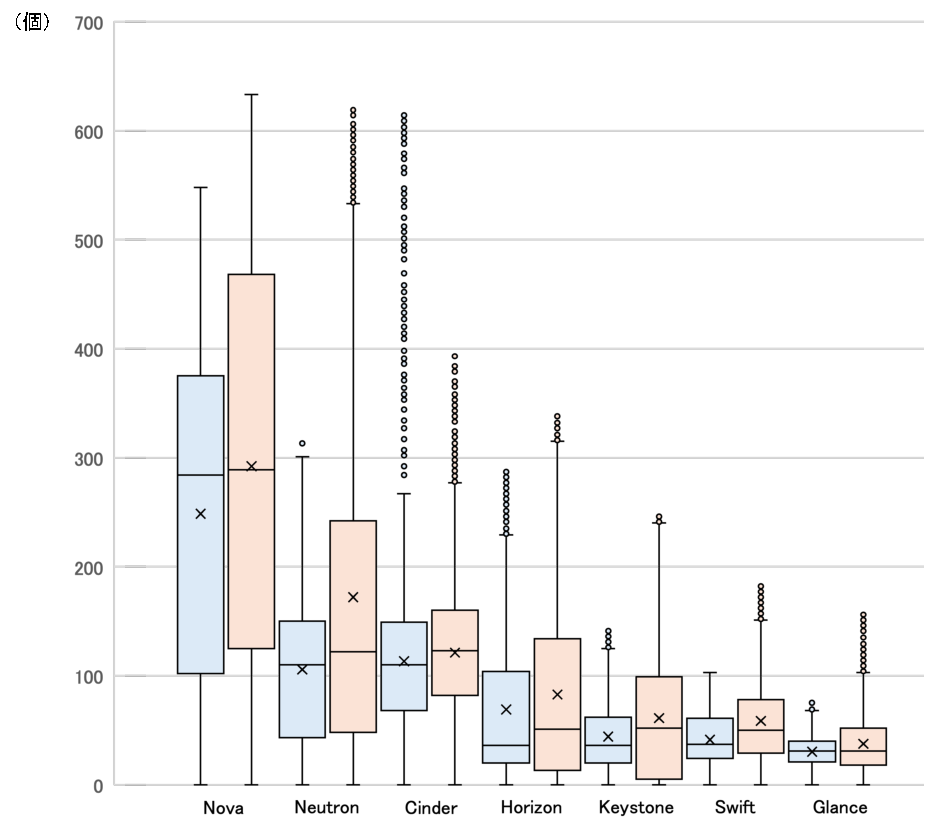
\includegraphics[width=0.9\linewidth]{@BSthesis2024_Kawasaki/BSthesis2024_Kawasaki_fig/task_distribution.pdf}}
\caption{1日ごとの未完了のコードレビュー票の件数と未完了の修正要求の件数の分布(左:未完了のコードレビュー票, 右:未完了の修正要求)}
\label{fig:task_distribution}
\end{figure}
%-------------------

表\ref{table:mann_whitney}は1日ごとの未完了のコードレビューの件数と未完了の修正要求の件数の分布に対して実施したMann-WhitneyのU検定の結果を示している.有意水準1\%において検定を行った結果,全てのプロジェクトにおいて,両者の分布間に統計的に有意な差が認められた.

%-----------------------
\begin{table}[t]
\centering
  \caption{1日ごとの未完了のコードレビュー票の件数と未完了の修正要求の件数の分布の差異}
  \label{table:mann_whitney}
  \scalebox{1.0}{   
  \begin{tabular}{l|r}  \hline \hline
    \multicolumn{1}{c|}{プロジェクト} & \multicolumn{1}{c}{p値}\\ \hline
    Neutron & $< 0.01$\\ 
    Nova & $< 0.01$\\ 
    Glance & $< 0.01$\\ 
    Cinder & $< 0.01$\\ 
    Swift & $< 0.01$\\ 
    Horizon & $< 0.01$\\ 
    Keystone & $< 0.01$\\ \hline
  \end{tabular}
  }
\end{table}
%-----------------------

次に,図\ref{fig:task_transition}は対象とする7プロジェクトに含まれる,未完了のコードレビュー票と未完了の修正要求の1日ごとの件数の推移を示す.2014年半ば頃から2017年までは未完了の修正要求の件数が未完了のコードレビュー票の件数に比べて特に多いことが確認できる.一方で,2017年頃,および2020年から2021年は未完了の修正要求の件数が未完了のコードレビュー票の件数に比べて特に少ないことが確認できる.また,図\ref{fig:request_per_pr}は式\ref{formula:relative}で示す,未完了の修正要求の件数と未完了のコードレビュー票の件数をそれぞれの平均の件数で除算した相対的な値(以降,未完了の件数の相対値)の推移を示す.

%-------------------
\begin{figure}[t]
\centerline{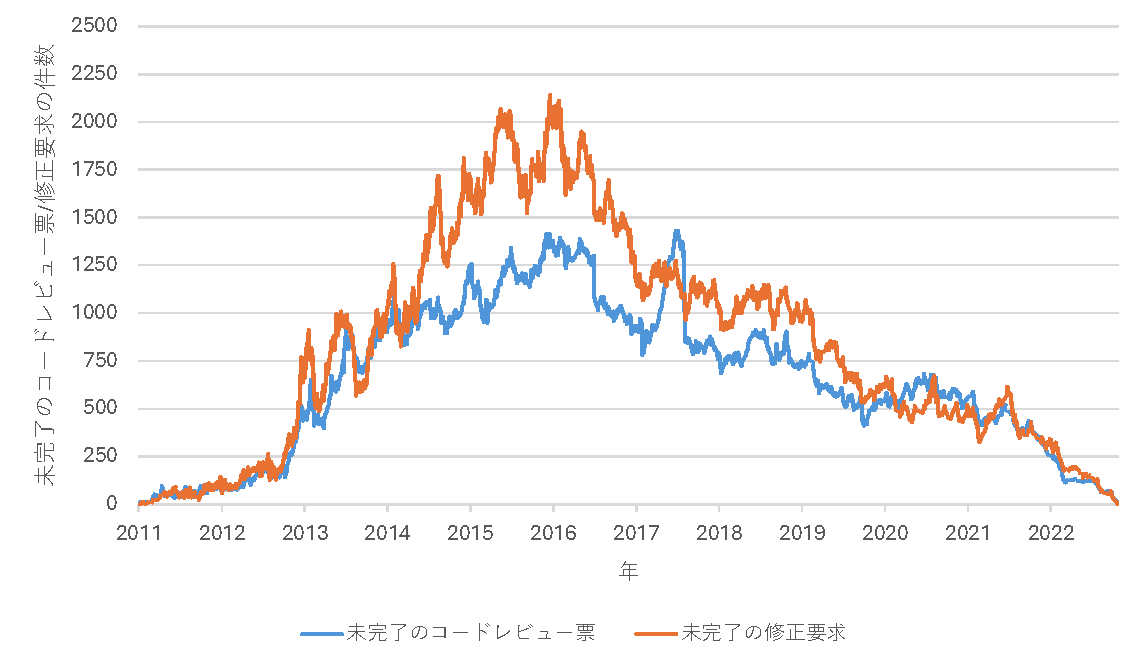
\includegraphics[width=1.0\linewidth]{@BSthesis2024_Kawasaki/BSthesis2024_Kawasaki_fig/task_transition.pdf}}
\caption{未完了のコードレビュー票の件数と未完了の修正要求の件数の推移}
\label{fig:task_transition}
\end{figure}
%-------------------

%-------------------
\begin{figure}[t]
\centerline{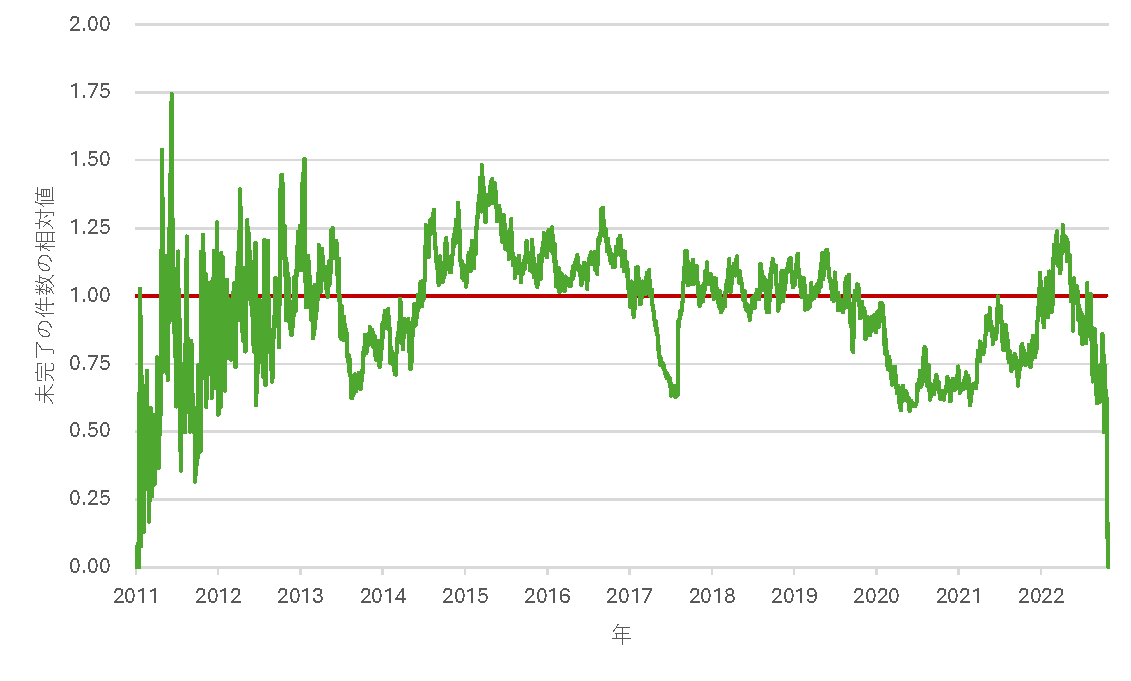
\includegraphics[width=1.0\linewidth]{@BSthesis2024_Kawasaki/BSthesis2024_Kawasaki_fig/request_per_pr.pdf}}
\caption{未完了の件数の相対値の推移}
\label{fig:request_per_pr}
\end{figure}
%-------------------

%-----------------------
\begin{equation}
未完了の件数の相対値 = \frac{\frac{該当日の未完了の修正要求の件数}{未完了の修正要求の平均件数}}{\frac{該当日の未完了のコードレビュー票の件数}{未完了のコードレビュー票の平均件数}} \label{formula:relative}
\end{equation}
%-----------------------

未完了の件数の相対値は,値の大小によって3つの通りに解釈可能である.

\begin{itemize}
\item $未完了の件数の相対値 > 1$: 1日の平均と比べて未完了の修正要求の件数が多い
\item $未完了の件数の相対値 = 1$: 1日の平均と比べて未完了の修正要求の件数が同程度
\item $未完了の件数の相対値 < 1$: 1日の平均と比べて未完了の修正要求の件数が少ない
\end{itemize}

したがって,図\ref{fig:request_per_pr}から,2014年の半ば頃から2017年頃は未完了の修正要求の件数が多いことが確認できる.一方で,2013年半ば頃から2014年半ば頃や2017年半ば,2020年から2022年は未完了の修正要求の件数が少ないことが確認できる.これらの結果から,コードレビュー票に投稿された未完了の修正要求の件数は時間によって変動することが示唆される.また,詳しい結果の議論については,\ref{subsec:utility}節で行う.

また,図\ref{fig:standard_deviation}は未完了のコードレビュー票に含まれる未完了の修正要求の平均値と標準偏差の推移を示す.ほぼ全ての期間において,平均値が1から2程度,標準偏差が2から3程度であることが確認できる.平均値に対する標準偏差の値が大きいことから,未完了の修正要求が多く投稿されているコードレビュー票と,あまり投稿されていないコードレビュー票が常に存在することが示唆される.また,この結果についても詳しい議論は\ref{subsec:utility}節で行う.

%-------------------
\begin{figure}[t]
\centerline{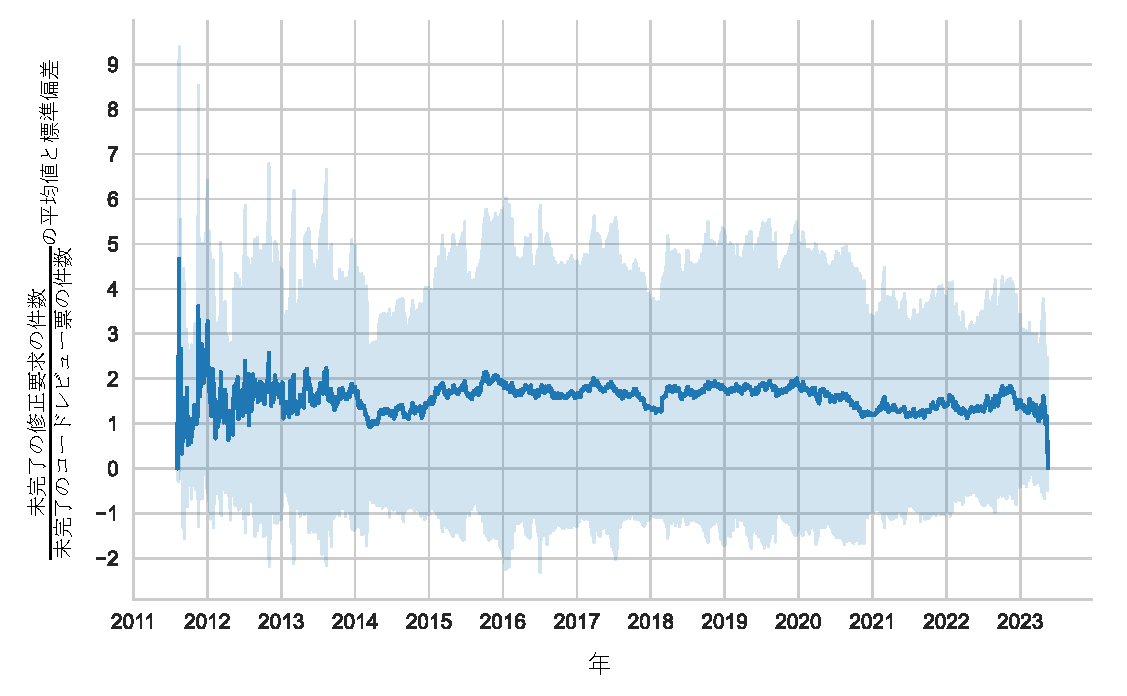
\includegraphics[width=1.0\linewidth]{@BSthesis2024_Kawasaki/BSthesis2024_Kawasaki_fig/standard_deviation.pdf}}
\caption{未完了のコードレビュー票に投稿された未完了の修正要求の件数の平均値と標準偏差の推移}
\label{fig:standard_deviation}
\end{figure}
%-------------------

%%%%%%%%%%%%%%%%%%%%%%%%%%%%%%%%%%%%%%%%%%
%7章 考察
\chapter{考察}\label{chap:discussion}
%%%%%%%%%%%%%%%%%%%%%%%%%%%%%%%%%%%%%%%%%%

\section{修正要求単位でのコードレビューのタスクの完了状況追跡手法は有用か}\label{subsec:utility}
図\ref{fig:request_per_pr}より,対象とするデータセットが同一であっても,コードレビュー票に投稿された未完了の修正要求の件数は時間によって異なることを確認した.また,図\ref{fig:standard_deviation}により,対象とする日が同一であっても,コードレビュー票に投稿された未完了の修正要求の件数はコードレビュー票ごとに異なることを確認した.仮に全てのコードレビュー票において,投稿される修正要求の数が同一であれば,修正要求単位でのタスクの完了状況の追跡は不要であると考えられる.しかし,時系列的な全体傾向においても,日次での個別の傾向においても,投稿された未完了の修正要求の件数にはコードレビュー票ごとに差異があることが分かる.

また,表\ref{table:close_time}はクローズまでに投稿された修正要求が0件から9件であったコードレビュー票について,そのクローズまでに要した時間の平均値と中央値を示している.修正要求の件数が増加するほど,クローズまでの所用時間の平均値,および中央値が大きくなることが確認できる.

これらの知見から,修正要求単位でタスクを抽出することで,従来では困難であった個々のコードレビュー票ごとのタスクの重みの比較やより詳細なタスクの完了状況の追跡が可能になることが示唆された.

%-----------------------
\begin{table}[t]
\centering
  \caption{修正要求の件数ごとのコードレビュー票のクローズ時間}
  \label{table:close_time}
  \scalebox{0.89}{   
  \begin{tabular}{r|r|r|r}  \hline \hline
    \multicolumn{1}{c|}{修正要求の件数} & \multicolumn{1}{c|}{コードレビュー票の件数} & \multicolumn{1}{c|}{クローズ時間の平均値(日)} & \multicolumn{1}{c}{クローズ時間の中央値(日)}\\ \hline
    0 & 42,328 & 14.26 & 3.13\\
    1 & 13,459 & 24.30 & 6.71\\
    2 & 8,349 & 30.41 & 9.09\\
    3 & 5,598 & 39.66 & 12.36\\
    4 & 4,088 & 42.98 & 14.97\\
    5 & 3,000 & 51.19 & 19.38\\
    6 & 2,196 & 54.22 & 21.27\\
    7 & 1,699 & 61.35 & 25.79\\
    8 & 1,348 & 68.29 & 27.40\\
    9 & 1,059 & 76.49 & 34.32\\ \hline
  \end{tabular}
  }
\end{table}
%-----------------------

\section{妥当性の脅威}
\subsection{内的妥当性}
本研究ではレビューコメントが修正要求か否か,修正確認か否かを著者が目視によって判断している.目視による分類結果は,他者の判断基準によって分類が異なる可能性がある.しかし,元々修正要求,および修正確認は,検証者から開発者に向けて修正を依頼または確認したことを意思表示するためのコメントであり,他者に対して伝わりやすい併用な記述法であることが一般的である.したがって,著者の判断基準は他者の判断基準と大きく異ならず,修正要求,および修正確認の分類への影響は小さいと示唆される.

また,修正確認の定義としてGerritで提供されている承認を示す検証評価ラベル及び\textit{``lgtm''},\textit{``looks good''},\textit{``looks ok''}を含むコメント群を用いたが,実際には\textit{``good change''}や\textit{``thank you''}のような他の表現を用いた修正確認が存在する.しかし,定義した修正確認コメントの判別基準は,著者が分類したデータセットから修正確認を高い精度で抽出しており,他の表現を用いた修正確認による予測精度への影響は小さいと示唆される.

紐付けの定義として二つの定義を提示したが,実際には定義に基づかない紐付き方も存在する.しかし,二つの定義で紐づいた割合が高いことから他の紐づき方による分析結果への影響は小さいと示唆する.

\subsection{外的妥当性}
本研究では,OpenStackのコアコンポーネントの6つのプロジェクトと大規模プロジェクトであるHorizonを対象とした.対象として用いるプロジェクトや期間によっては予測精度や分析結果が異なることが示唆される.しかし,OpenStackプロジェクトでは,各コードレビュー票に対する開発者からのコメント投稿数が多いため,データセットとするプロジェクトや期間の変更による予測精度や分析結果への影響は小さいと示唆する.

%%%%%%%%%%%%%%%%%%%%%%%%%%%%%%%%%%%%%%%%%%
%8章 おわりに
\chapter{おわりに}\label{chap:conclusion}
%%%%%%%%%%%%%%%%%%%%%%%%%%%%%%%%%%%%%%%%%%

本研究では,コードレビュー票に投稿された修正要求,および修正確認に基づいたコードレビューのタスクの完了状況の追跡手法を提案し,3つのRQを検証した.

\begin{itemize}
\item RQ1: \RQOne
\item RQ2: \RQTwo
\item RQ3: \RQThree
\end{itemize}

RQ1では,目視調査,およびBERTを用いてレビューコメントから修正要求を抽出することが可能であるかを検証した.その結果,目視で分類したデータセットを用いて構築したBERTのモデルにより,レビューコメントから修正要求を高い精度で抽出することが可能であることを確認した.

RQ2では,目視調査,およびパターンマッチを用いてレビューコメントから修正確認を抽出することが可能であるかを検証した.その結果,目視で得られた特徴に基づいて作成したパターンを用いることで,レビューコメントから修正確認を高い精度で抽出することが可能であることを確認した.

RQ3では,定義した紐付け手法を用いて修正要求と修正確認を紐づけることが可能であるかを検証した.その結果,定義した紐付け手法は高い割合で修正要求と修正確認を紐づけることが可能であることを確認した.また,定義した紐付け手法に基づいて分析対象区間内の修正要求の完了度合いの分布と推移を調査したところ,従来のコードレビュー票の分布や推移と異なっていることを確認した.

本研究で提案した修正要求単位でのコードレビューのタスクの完了状況追跡手法により,個々のコードレビュー票のタスクの完了状況を詳細に把握することが可能となる.この手法を用いることで,ソフトウェアの開発プロセスの効率化に貢献することを期待する.

\begin{acknowledgements}
本研究を進めるに当たって,多くの方々から御指導,御協力を賜りましたことを,ここに深く感謝を申し上げます.

まず,指導教員である和歌山大学システム工学部伊原彰紀准教授に,心より感謝申し上げます.研究室配属から現在に至るまで,研究の方向性,論文執筆の作法,学会発表など,数多くの御指導を賜りました.また,研究発表の機会を与えていただき,多くの研究者との貴重な交流の場を設けていただきました.ここに深く感謝の意を表します.

次に,本研究を進めるにあたり,多大なご協力をいただきました和歌山大学システム工学研究科上中瑞稀氏に厚く御礼申し上げます.研究に関して,御協力,御助言をいただきました.

また,和歌山大学ソーシャルソフトウェア工学研究室の方々には,普段から多大な御協力,御助言をいただきました.特に,ソーシャルソフトウェア工学研究室の同期の皆様には,研究面だけでなく,学生生活全般にわたって御支援いただき,充実した研究生活を送ることができました.心より感謝申し上げます.

最後に,研究生活を常に支え,励まし続けてくれた家族に対し,深い感謝の意を表します.
\end{acknowledgements}

%================
%\section*{参考文献}
%================
\bibliographystyle{junsrt}
\bibliography{@BSthesis2024_Kawasaki/BSthesis2024_Kawasaki}

\end{document}
